\begin{figure}[h]
        \centering
        \begin{subfigure}[b]{0.5\textwidth}
                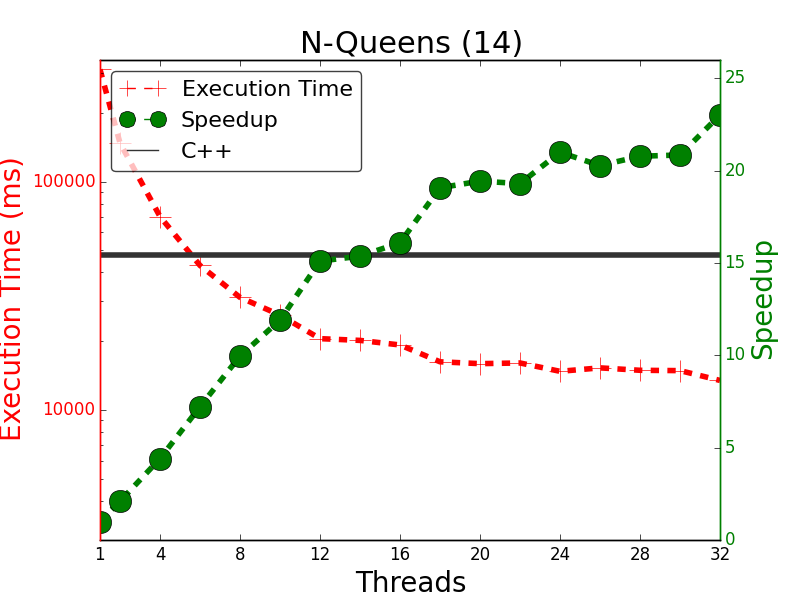
\includegraphics[width=\textwidth]{experiments/scalability/scale-8queens-14.png}
                \caption{Initial database. Replace axiom instantiated at the
                   \code{@3} root node.}
                   \label{fig:implementation:scale_queens}
        \end{subfigure}%
        ~
        \begin{subfigure}[b]{0.5\textwidth}
                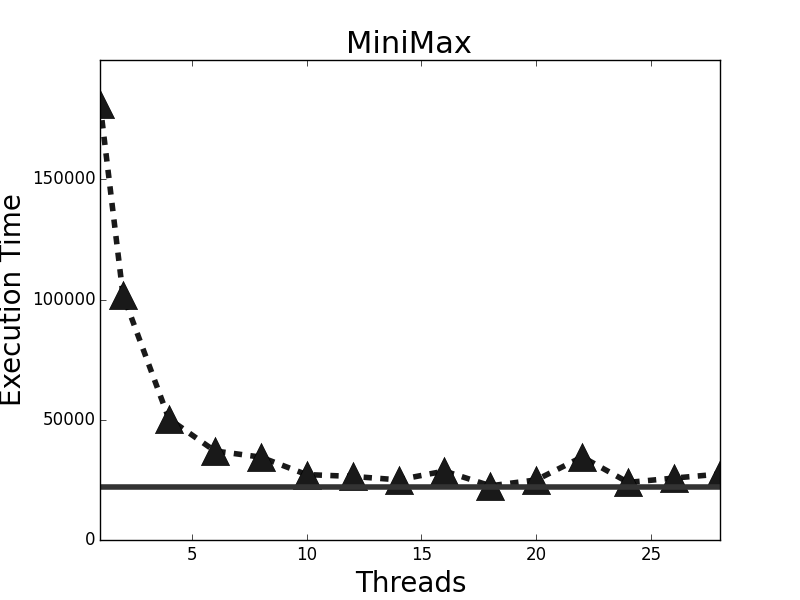
\includegraphics[width=\textwidth]{experiments/scalability/scale-min-max-tictactoe.png}

                \caption{After applying rule 3 at node \code{@3}. The
                \code{replace} fact is \emph{sent} (or derived at) to node
                \code{@5}.}

                \label{fig:implementation:scale_minmax}
        \end{subfigure}\\
        \begin{subfigure}[b]{0.5\textwidth}
                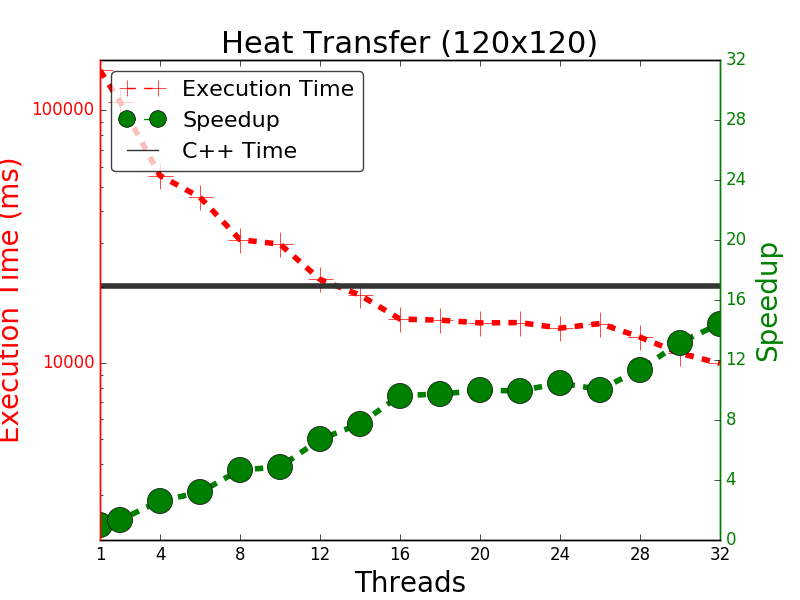
\includegraphics[width=\textwidth]{experiments/scalability/scale-new-heat-transfer-120.png}
                \caption{Initial database. Replace axiom instantiated at the
                   \code{@3} root node.}
                   \label{fig:implementation:scale_heat}
        \end{subfigure}%
        ~
        \begin{subfigure}[b]{0.5\textwidth}
                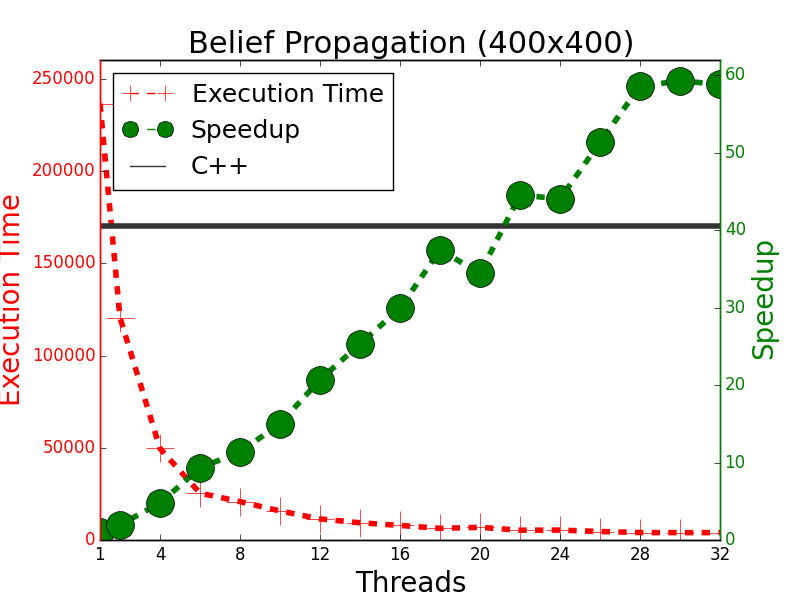
\includegraphics[width=\textwidth]{experiments/scalability/scale-belief-propagation-400.png}

                \caption{After applying rule 3 at node \code{@3}. The
                \code{replace} fact is \emph{sent} (or derived at) to node
                \code{@5}.}

                \label{fig:implementation:scale_bp}
        \end{subfigure}\\
        \caption{An execution trace for the binary tree dictionary
           algorithm. The first argument of each fact was dropped and the
           address of the node was placed beside it.}
        \label{fig:implementation:scale1}
\end{figure}
